\chapter{Présentation}

	\section{Présentation générale de l'application}

        Magic Book est un éditeur de livre permettant de créer un livre à choix multiple pouvant contenir des conditions pour certains d'entre eux, des choix aléatoires, des combats, etc. L'utilisateur peut donc créer des paragraphes, appelés des "noeuds", reliés entre eux par des liens. Ces liens peuvent être bloqués par des prérequis, permettant ainsi que l'utilisateur rajoute de la difficulté dans l'histoire. L'ajout de personnages, d'items et de compétences sont aussi disponibles, répondant au mieux à l'imagination de l'utilisateur. Une fois le livre créé, l'utilisateur peut alors obtenir une estimation de la difficulté du livre en choisissant l'option correspondante dans la barre de menu en haut. Cette difficulté est ensuite affichée dans le panel des stats. Une option "Jouer" est également disponible, permettant ainsi de jouer à l'histoire créée. Enfin, il est également possible d'exporter le livre dans un format texte. Bien entendu, il est possible d'enregistrer le livre afin de le réouvrir pour continuer l'édition de celui-ci.

	\section{Présentation de l'application}

		\begin{figure}[H]
			\centering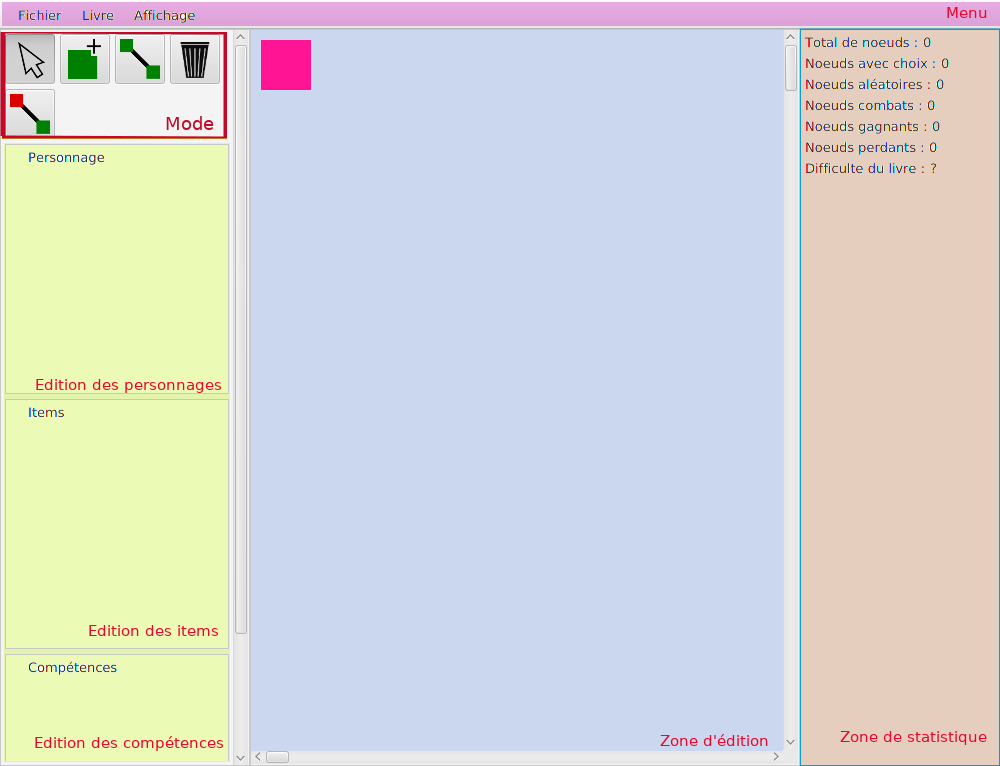
\includegraphics[width=0.7\textwidth, keepaspectratio]{img/magicBook.png}
		\end{figure}

		L'application comprend quatre parties. Un menu, permettant d'utiliser toutes les options de cette application, que cela soit pour sauvegarder ou charger un livre, pour afficher ou masquer les différentes zones de l'application ou encore, effectuer divers traitements sur le livre (estimer la difficulté, jouer, etc). On remarquera une zone en haut à gauche, contenant divers boutons permettant de sélectionner un mode (sélectionner, ajouter un noeud, etc). En dessous de ces boutons, des listes sont affichées. Celles-ci contiennent les personnages, items, compétences du livre actuel. Il y a ensuite la zone d'édition, au milieu. Cette zone contient les différents paragraphes du livre. La zone à droite permet à l'utilisateur d'avoir une vue globale sur son livre grâce à différentes statistiques : nombre de noeuds au total, nombre de noeuds en fonction de son type, difficulté du livre...

	\section{Informations supplémentaires}

		Actuellement certaines fonctionnalités ne sont pas complète, voici quelques précisions sur certaines d'entre elles :

		\begin{itemize}
			\item{Bien que différentes monnaies puissent être renseignées, tous les champs demandant un montant de monnaie se base sur celle qui aura pour ID "gold". Pour éviter les bugs il est mieux d'en avoir au moins une avec cette ID.}
			\item{Bien que l'on puisse renseigner les "shop" dans un noeud, ceux-ci n'apparaissent pas encore en jeu.}
			\item{Bien que l'on puisse renseigner l'usure d'un item, ceux-ci ne sont pas encore pris en compte dans le jeu.}
		\end{itemize}
